\documentclass[20pt,,margin=1in,innermargin=-4.5in,blockverticalspace=-0.25in]{tikzposter}
\geometry{paperwidth=42in, paperheight=34in}
\usepackage[utf8]{inputenc}
\usepackage{amsmath}
\usepackage{amsfonts}
\usepackage{amsthm}
\usepackage{amssymb}
\usepackage{mathrsfs}
\usepackage{graphicx}
\usepackage{adjustbox}
\usepackage{enumitem}
\usepackage[backend=biber,style=numeric]{biblatex}
\usepackage{SUtheme}

\usepackage{mwe} % for placeholder images

\addbibresource{refs.bib}

% set theme parameters
\tikzposterlatexaffectionproofoff
\usetheme{SUTheme}
\usecolorstyle{SUStyle}
\usetitlestyle{Filled}

\usepackage[scaled]{helvet}
\renewcommand\familydefault{\sfdefault} 
\usepackage[T1]{fontenc}


\title{Chelko, USA Network Traffic}
\author{Randy Heckard, Spencer Metz, Matthew Montney, Damien Rodriguez, Kevin Underwood}
\institute{Eastern Washington University}
\titlegraphic{
\includegraphics[width=0.16\textwidth]{images/ewu logo.jpg}}


% begin document
\begin{document}

\maketitle
\centering
\begin{columns}
    \column{0.32}
    \block{Introduction}{
    Using a real-time data analytics and logging tool, the Chelko team monitored network traffic for a Washington State County. The use of Open-source Intelligence (OSINT) and traffic logs were crucial to identifying malicious activity. Any occurrence of potentially malicious network traffic that had the potential to harm the computers and infrastructure was raised to PISCES and the Washington State Fusion Center.  
         \vspace{1em}
          \vspace{1em}
          \vspace{1em}
          \vspace{1em}
          \vspace{1em}
          \vspace{1em}
          \vspace{1em}
    \vspace{1em}


    }
    \block{Methods}{
    We used Kibana for monitoring traffic. Mantis was used for reporting anything we found suspicious. The way to find out if something is suspicious is to put the ips into other sites such as Talos, VirusTotal, Whois, and/or Abuse Ip Database. Looking at the massive amount of data coming in is daunting so applying filters is essential.
         \vspace{1em}
          \vspace{1em}
          \vspace{1em}
          \vspace{1em}
          
         
        
    \begin{tikzfigure}[Suspicious Results]
        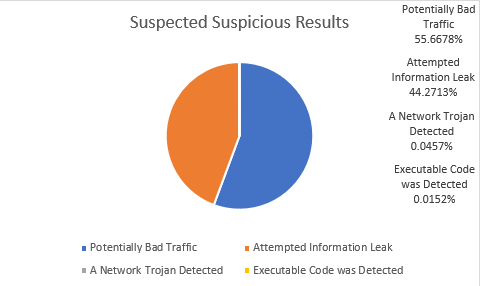
\includegraphics[width=1\linewidth]{images/graph1.PNG}
    \end{tikzfigure}
    }
    
    

    \column{0.36}
    \block{Observations}{ 
    Many alerts found over the course of the quarter were found to be a false positive.
    This is the result of a poorly optimized suricata, and little to no changing of any of the rules provided by it. In order to try and minimize false positives, we recommend going through the rules list of Suricata, and whitelisting IP’s that are official IP’s that are meant to communicate with the internal network.

    \begin{tikzfigure}[Top 30 alerts.]
        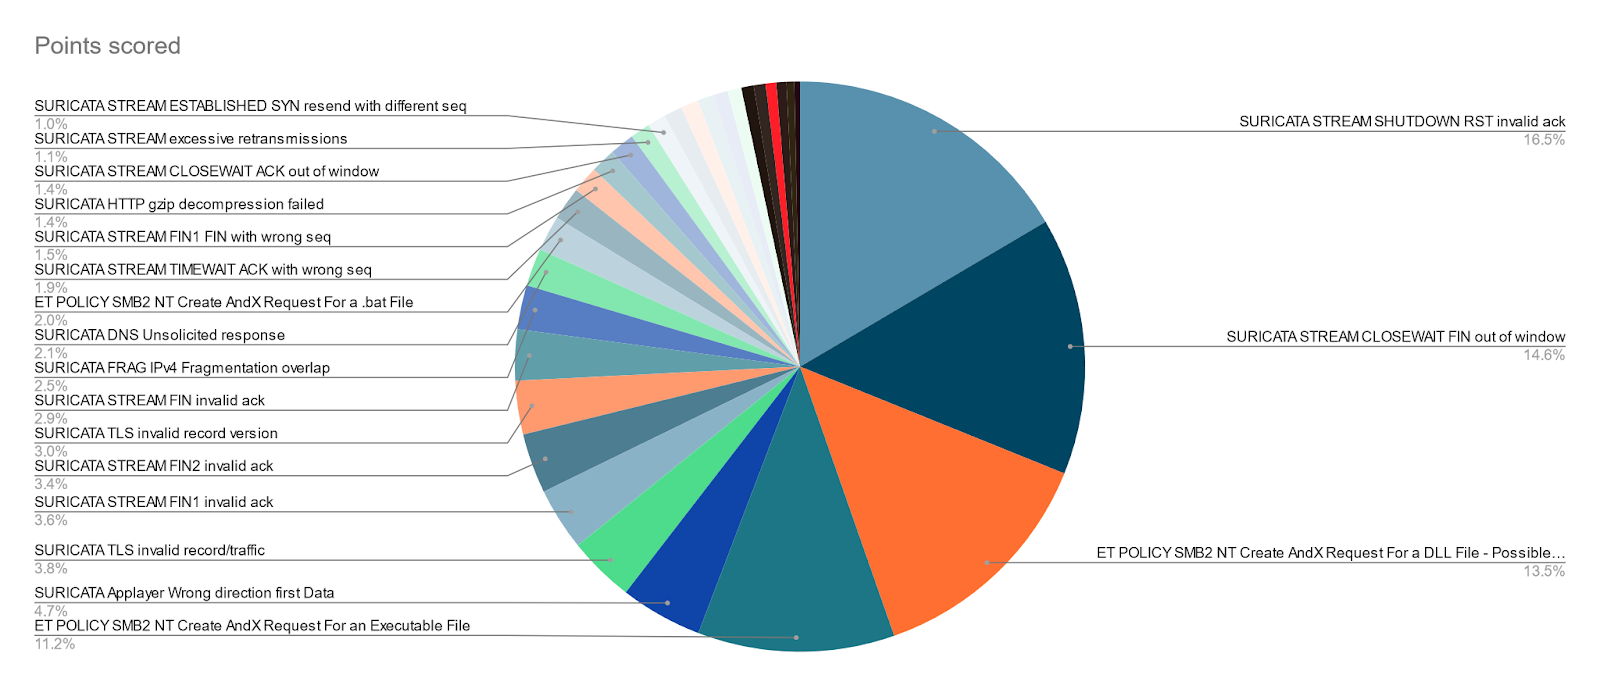
\includegraphics[width=1\linewidth]{images/top30alerts.png}
    \end{tikzfigure}

    \section{.onion}{
    What is it?
    URLs containing the .onion domain are websites that can't typically be accessed from mainstream web browsers. This area of the internet is known as the "Dark Web". The "Dark Web" and "Deep Web" are used interchangeably, but are not the same thing. The Dark Web is where certain websites reside that require special software to access. 
    
    \vspace{1em}
    What we found:
    At least three devices on a local network Regular requests to .onion and .to TLDs This Likely is someone accessing the deep web without TOR.
    }
    \section{SSH}{
    What is it?
        SSH connection attempts were flagged as outbound scans to an outside IP that we determined was the municipalities primary IT Security company.
    \vspace{1em}
    
    What we found:
    
    Regular outbound SSH scans. Same source IP communicating with multiple destination IPs. Probably Microsoft SQL server using SSH
    }
    \section{TROJAN Zeus GameOver}{
    What is it?
    
    GameOver Zeus is an extremely sophisticated type of malware designed specifically to steal banking and other credentials from the computers it infects. It's predominately spread through spam e-mail or phishing messages.
    \vspace{1em}
    
    What we found:

    This traffic occurred once a month and only happened once between different devices each time Was occurring on between devices on the network. this turned out to be a false positive that triggered a Suricata alert. 
    }
    }
    \vspace{1em}
    
    
    
    
    \column{0.32}
    \block{Results}{
    The results from our six weeks of monitoring were mostly false positive results. Over 90 percent of which were due to supposed improper configuration of Suricata rules. We recommend that the system administrators tune out certain rules, such as Generic Protocol Command Decode (which took up 90 percent of total results), to reduce the amount of false positives. For the .onion DNS queries, we recommend that traffic asking for those queries be disallowed internally. For the Network Trojan, we recommend a scorched earth approach, and completely wipe existing machines, replacing with backups. For instances such as the SSH connection attempts, we recommend that an extensive whitelist of official channels be created to help reduce the false positive flags as well.
    \vspace{1em}
    \vspace{1em}
    \vspace{1em}


    }

    \block{Resources}{
        A few of the tools we used:
        \begin{itemize}
        \item www.abuseipdb.com 
        \item whois.domaintools.com 
        \item www.virustotal.com/gui/home/search
        \end{itemize}
            \vspace{1em}
    \vspace{1em}
        \begin{tikzfigure}[Overall Traffic]
            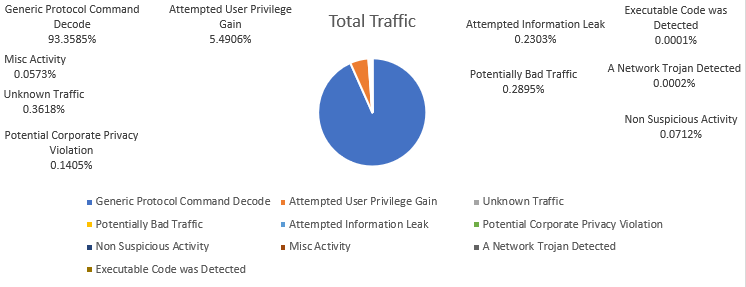
\includegraphics[width=1\linewidth]{images/graph3.PNG}
        \end{tikzfigure}
        
            \vspace{1em}
    \vspace{1em}
        
        }
        
        \vspace{1em}
        \vspace{1em}
        
        \vspace{1em}
        \block{Acknowledgements}{
        Youtube: https://www.youtube.com/watch?v=rQD1N-DOK-I
        \begin{tikzfigure}[Overall Traffic]
        
\includegraphics[width=0.3\linewidth]{images/qrcode1615930266.png}
         \end{tikzfigure}
                 \vspace{1em}
        \vspace{1em}
        
        \vspace{1em}
    \vspace{1em}
        
        }
        
\end{columns}
    \block{Security Operations Analyst
    - CSCD496
    - Dr Stuart Steiner
    - Winter 2021
    - Eastern Washington University - Department of Computer Science
}{
}
\end{document}
